\begin{figure}[ht]
\centering
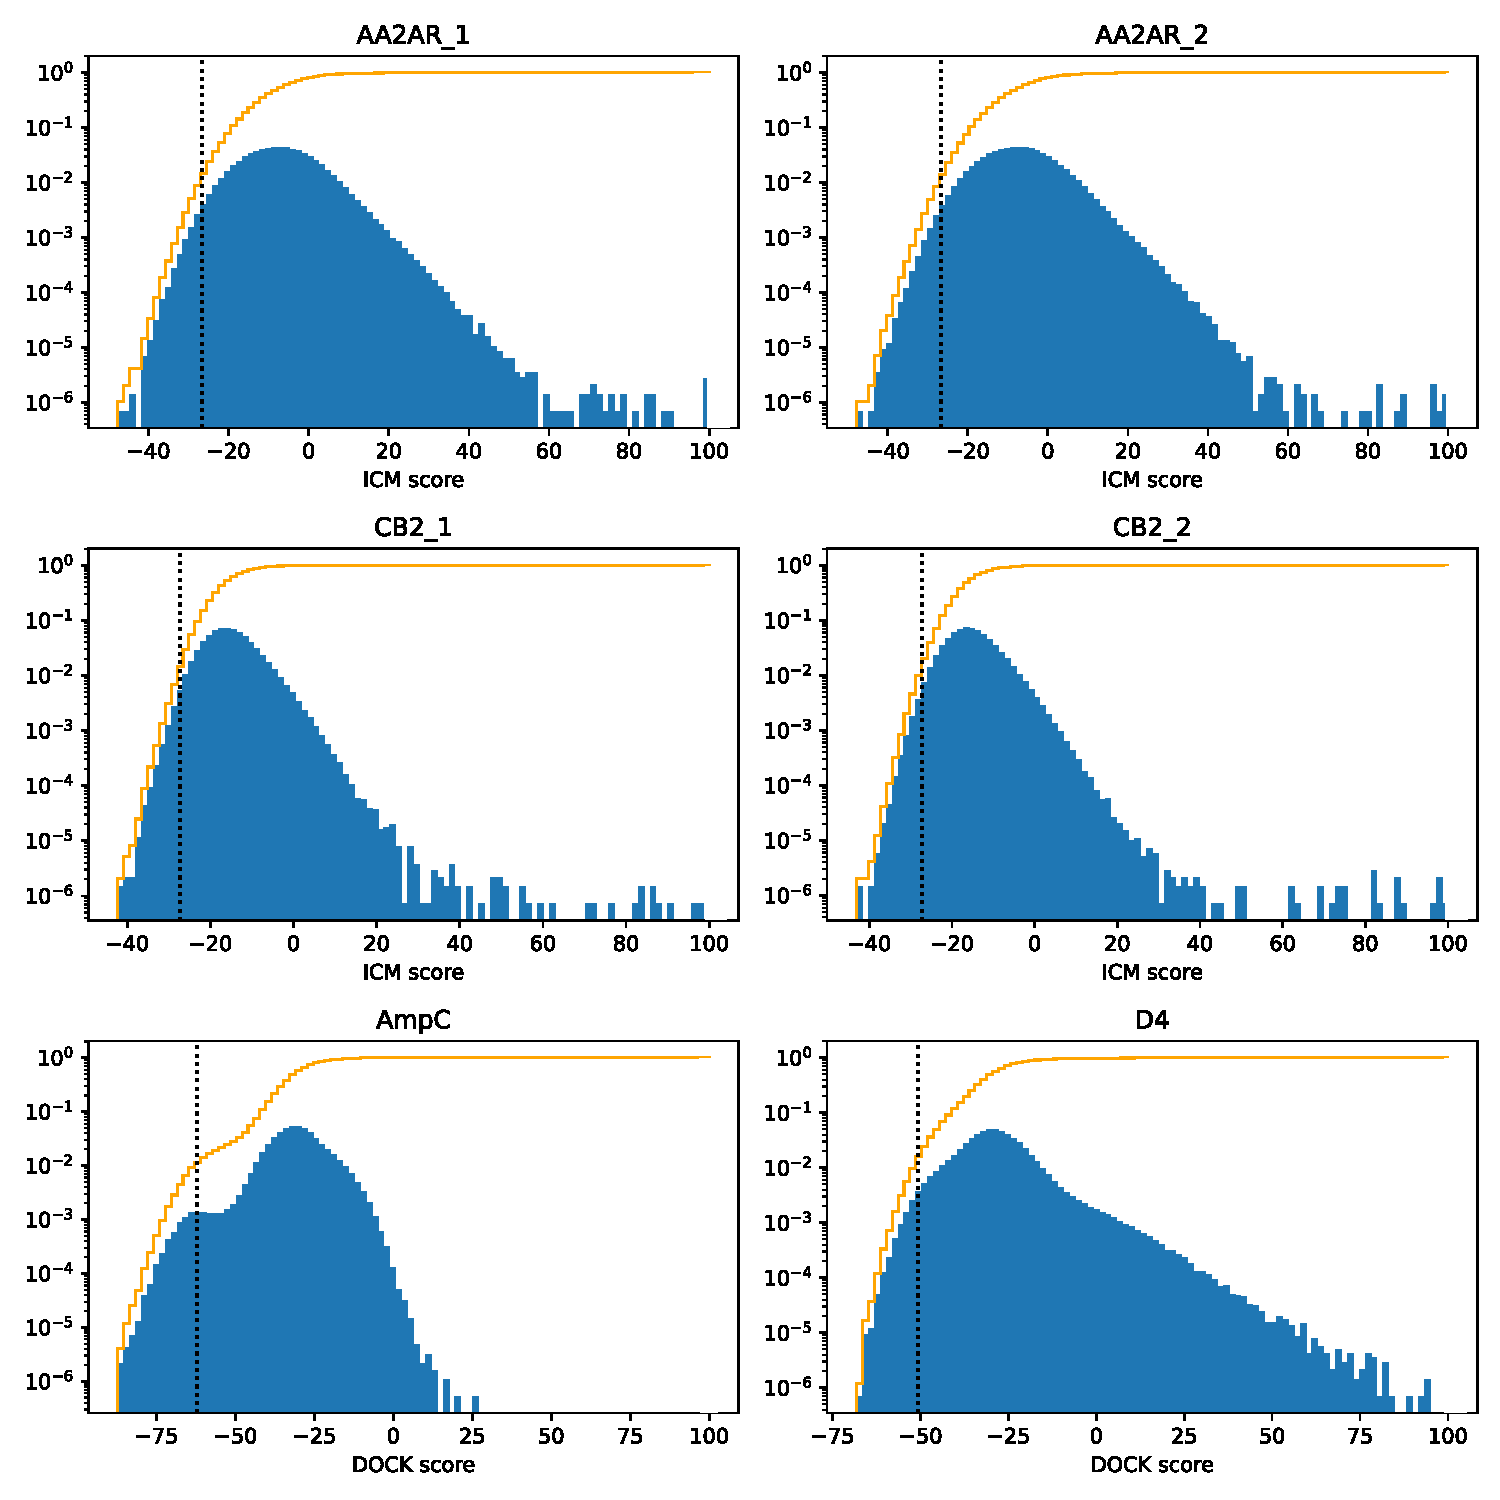
\includegraphics[width=1.0\textwidth]{figures/figure_1_scores_distribution_v3.pdf}
\caption{Distributions of scores for datasets used in the study. Histogram (blue) shows log-scale score distribution, while plot (orange) shows cumulative distribution of scores. Vertical line (black) shows cutoff for top-1\% of scores.}
\label{fig:fig_1_distribution}
\end{figure}


\begin{figure}[ht]
\centering
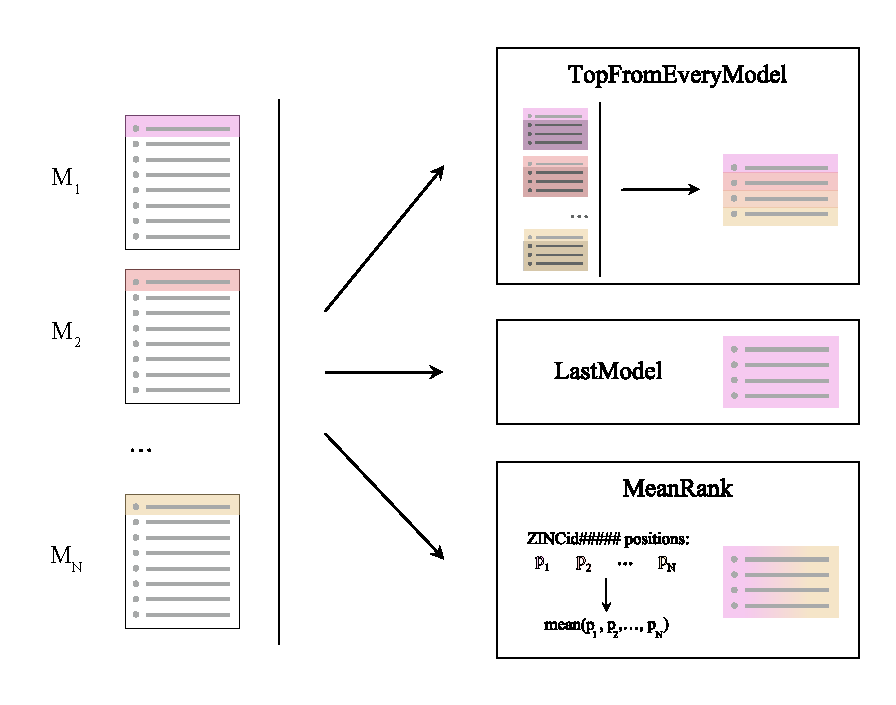
\includegraphics[width=1.0\textwidth]{figures/Figure_2_v4.pdf}
\caption{Overview of the active learning ranking schemes.}
\label{fig:fig_2_scheme}
\end{figure}


\begin{figure}[ht]
\centering
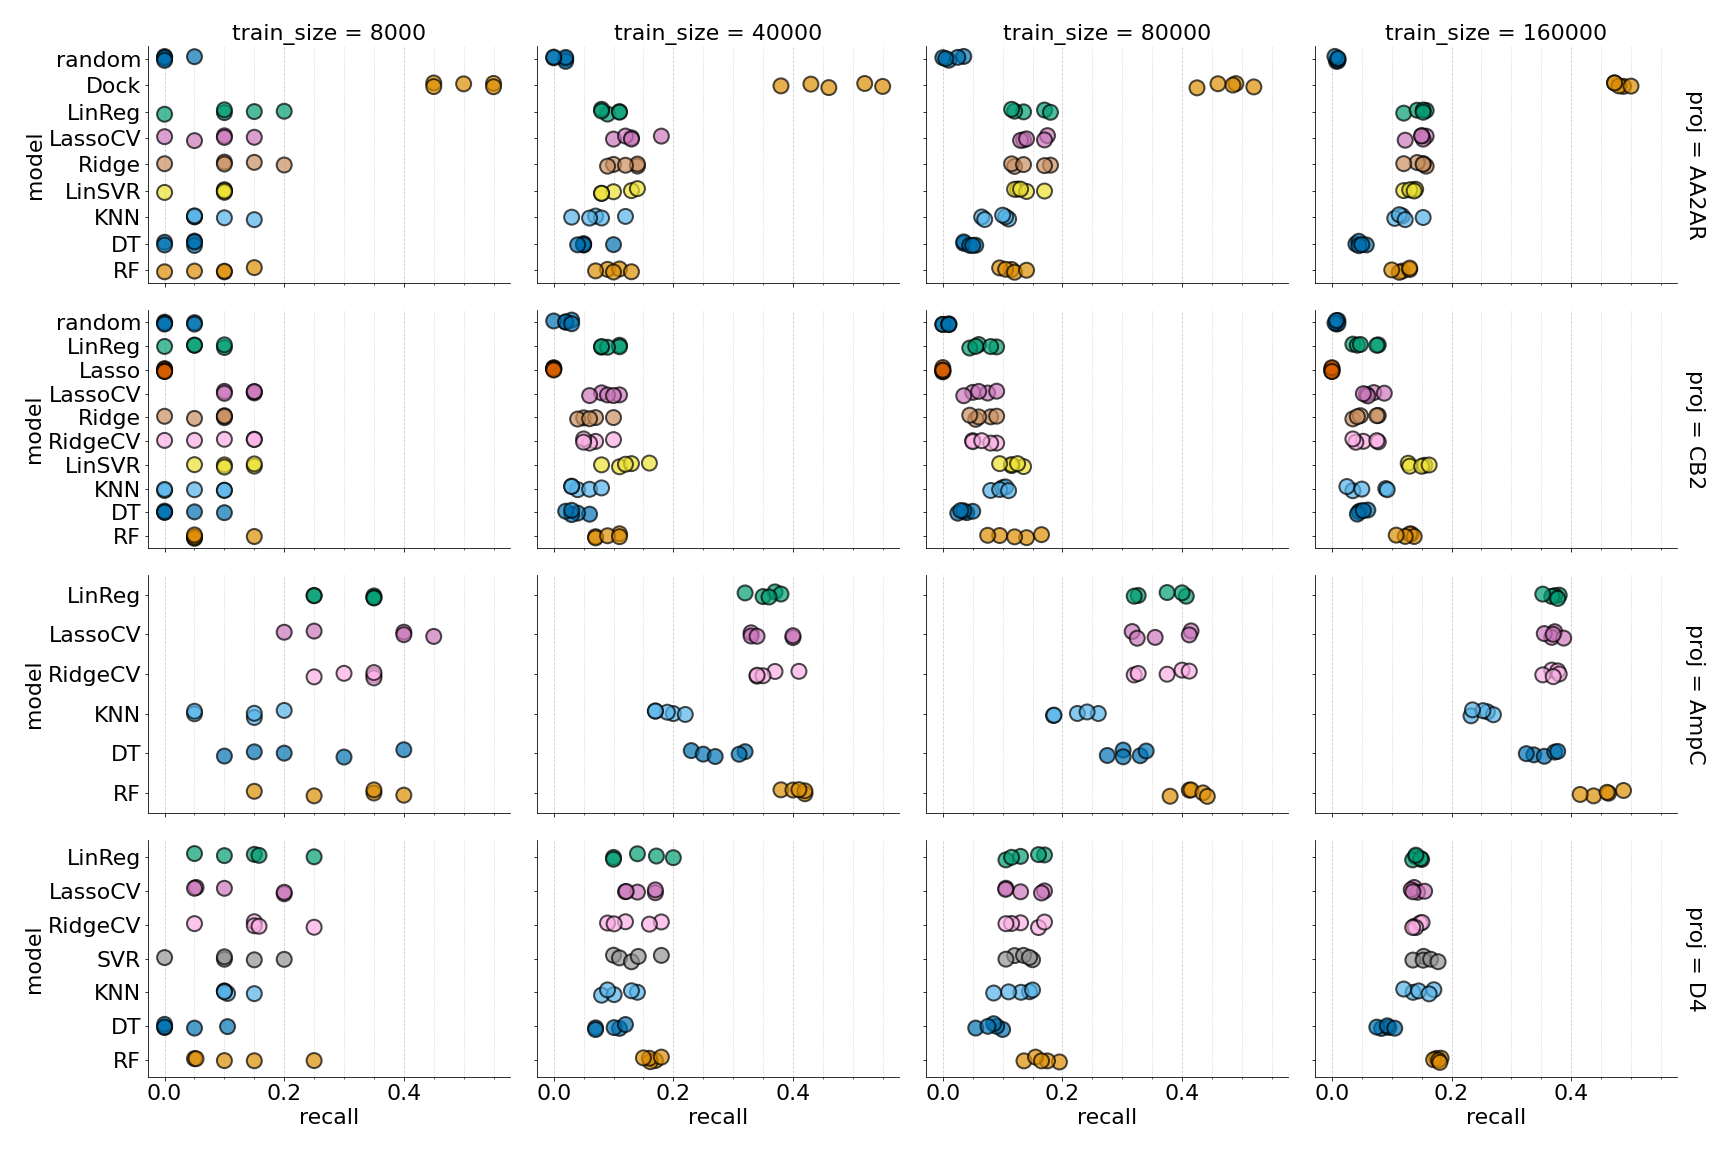
\includegraphics[width=1.0\textwidth]{figures/figure_3_single-shot-performance.png}
\caption{Model performance for multiple regression models and their baselines on 4 datasets present in the study. \texttt{recall\_score} shows the share of interception of top-1\% of the regressor's predictions with the actual top-1\%, sorted by docking score}
\label{fig:fig_3_singleshot}
\end{figure}


\begin{figure}[ht]
\centering
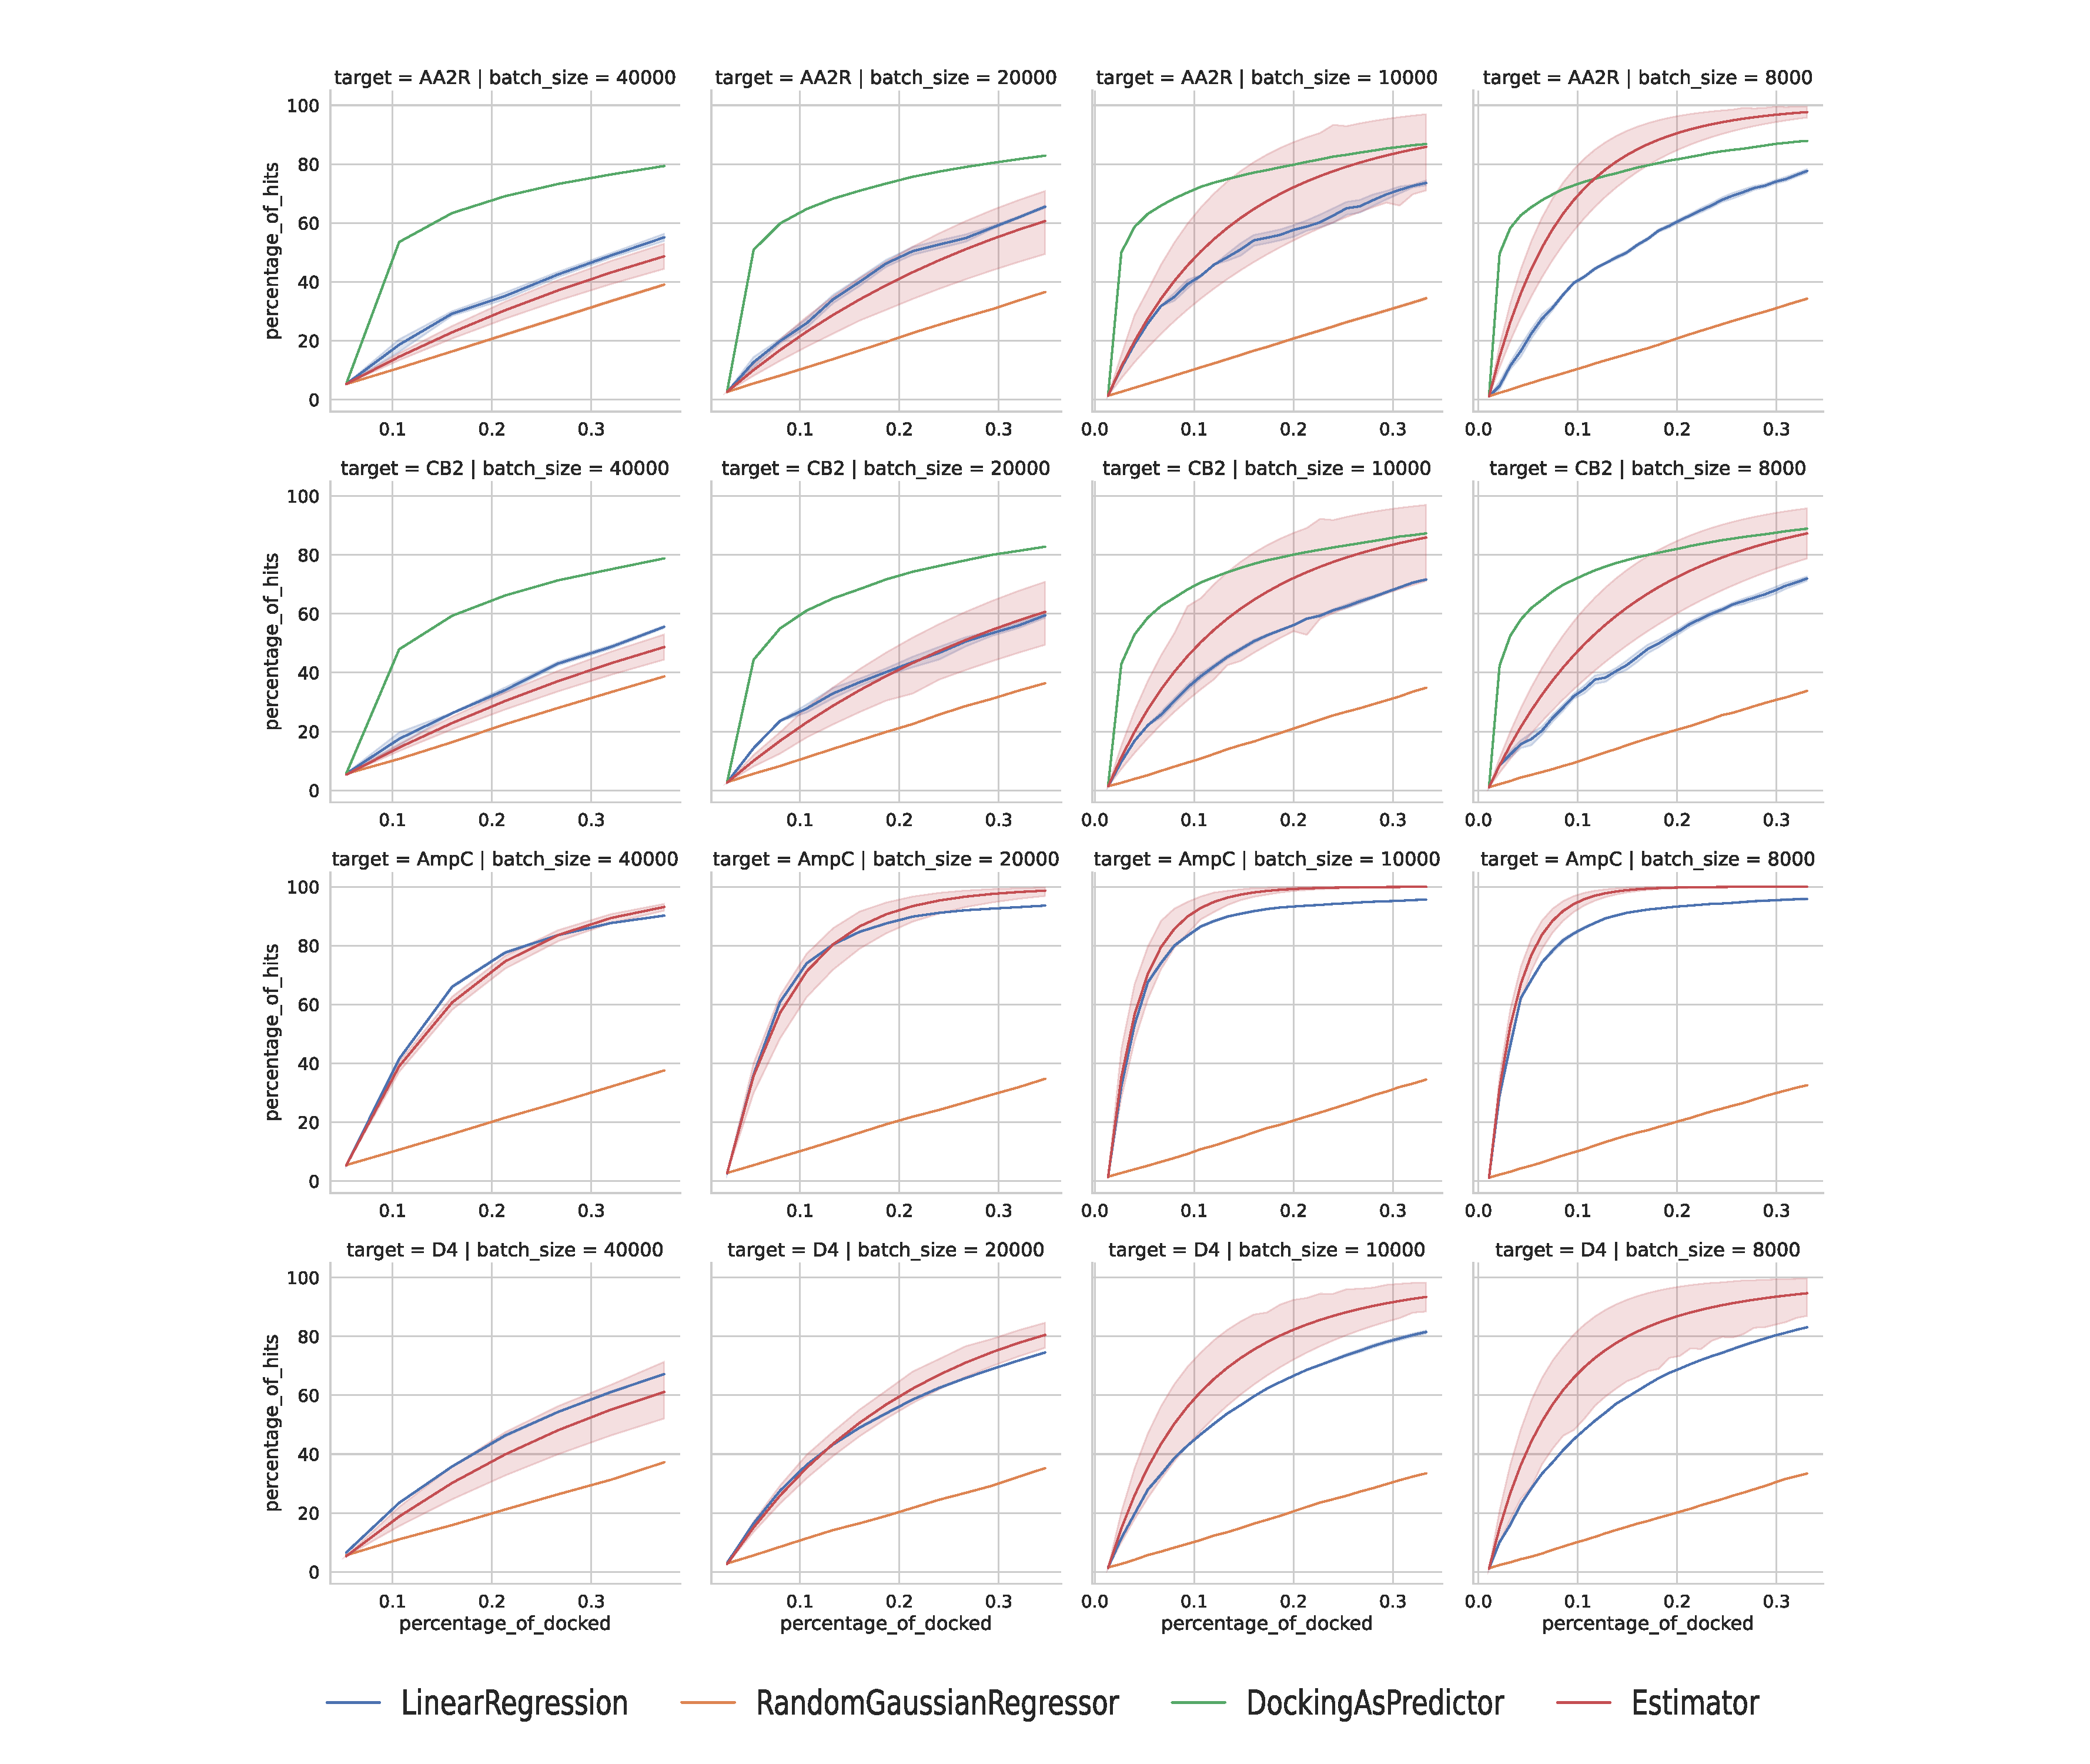
\includegraphics[width=1.0\textwidth]{figures/figure_4_iterations.pdf}
\caption{Model performance for multiple regression models and their baselines on 4 datasets present in the study. \texttt{recall\_score} shows the share of interception of top-1\% of the regressor's predictions with the actual top-1\%, sorted by docking score}
\label{fig:fig_4_extrapolation}
\end{figure}


\begin{figure}[ht]
\centering
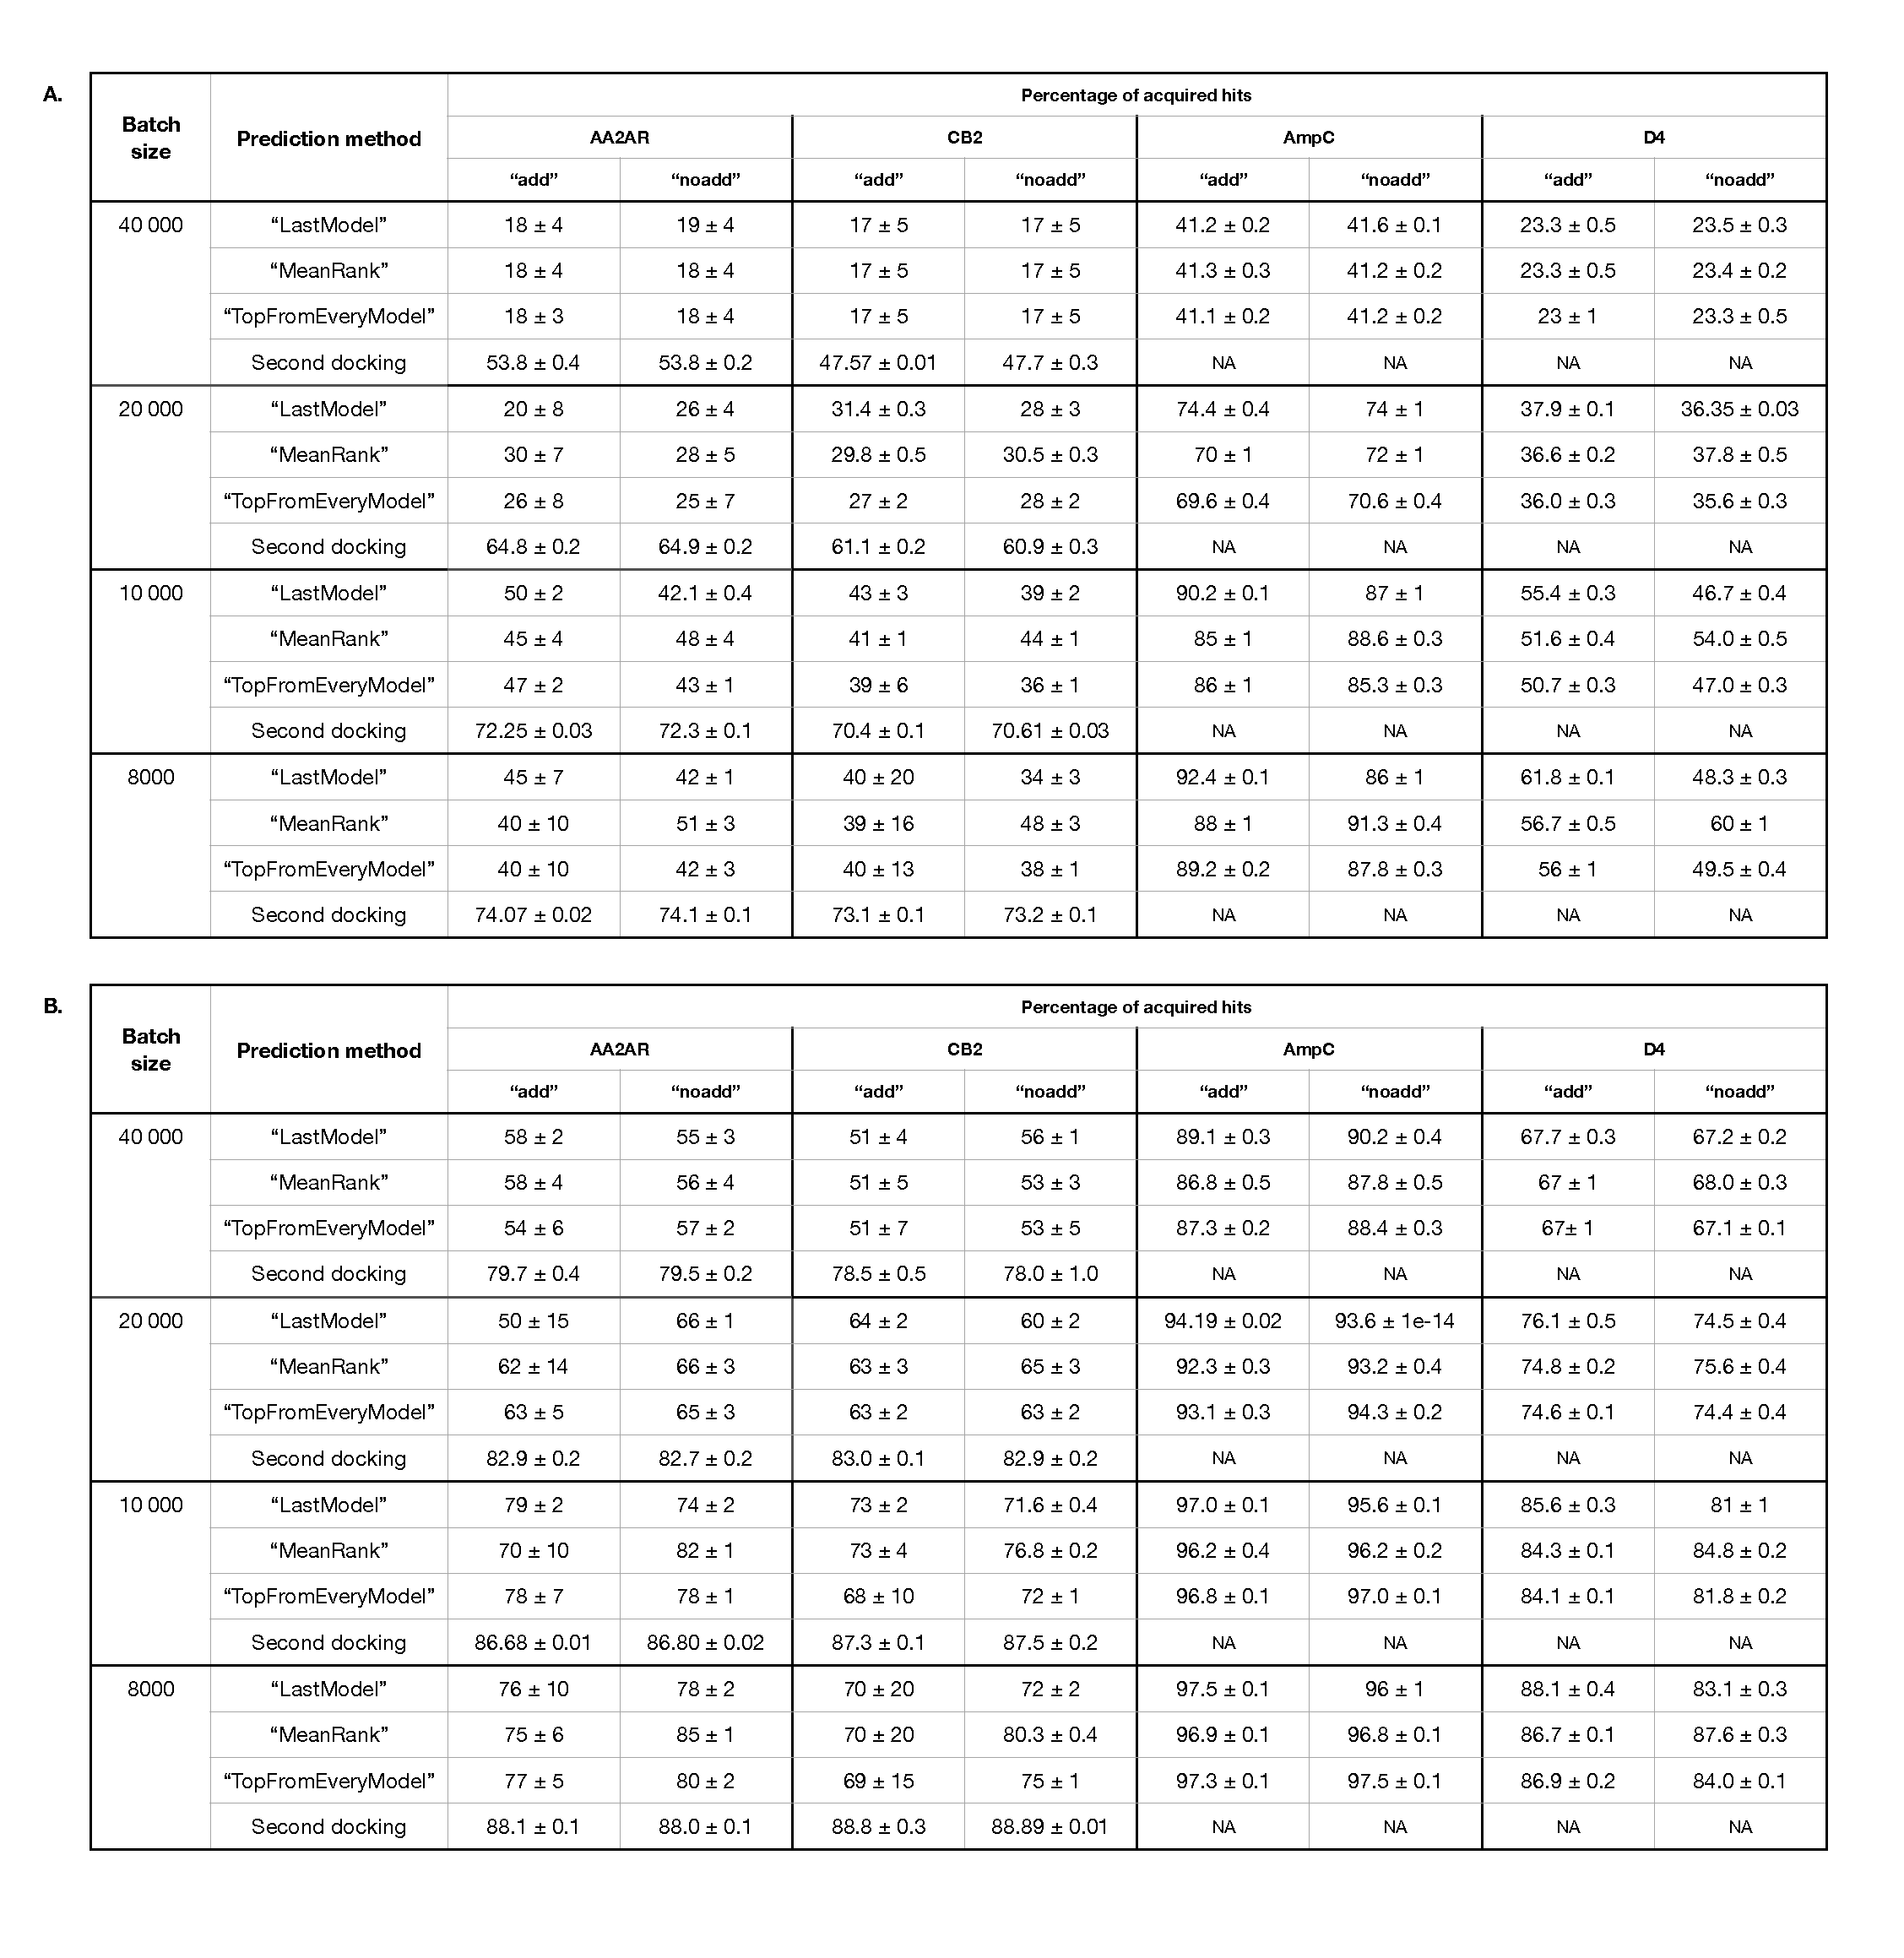
\includegraphics[width=1.0\textwidth]{tables/table_1_full.pdf}
\caption{Active learning regimes performance at a) early (after 10\% library screened) recall; b) late (after 30\% library screened) recall.}
\label{tab:tab_1_activelearning}
\end{figure}
